%***********************************************************************
% Lab Report Template
% R. W. Melton
% May 19, 2019
% August 24, 2020
% January 4, 2021
%***********************************************************************
%Modify the following macros to set document property values
%used for cover sheet (title page) and page header
\newcommand{\CourseNumber}{CMPE 160.01}
\newcommand{\CourseName}{Digital System Design I}
\newcommand{\SemesterName}{Spring 2023}
\newcommand{\SemesterCode}{2235}
\newcommand{\LabExNum}{8}
\newcommand{\LabExTitle}{Design and Simulation of a Moore State Machine}
\newcommand{\StudentName}{Adam Schultzer}
\newcommand{\DateSubmit}{3/28/2024}
\newcommand{\LabSection}{3}
\newcommand{\LabInstructor}{Mr. Lange}
\newcommand{\TAa}{Andy Lin}
\newcommand{\TAb}{Christian Rockwell}
\newcommand{\TAc}{Ruhan Syed}
\newcommand{\TAd}{Matthew Tosi}
\newcommand{\LectureSection}{01}
\newcommand{\LectureInstructor}{Richard Cliver}
%End macros for document property values
%***********************************************************************
\title{Lab Ex. \LabExNum\ Report}
\author{\StudentName}
\date{\DateSubmit}
\makeatletter %make \title, \author, and \date available with \@
\newcommand{\FontSize}{12}
\newcommand{\FontUnit}{pt}
\newcommand{\HeadSize}{\dimexpr \FontSize\FontUnit + 2pt \relax}
\documentclass[\FontSize\FontUnit,letterpaper,oneside]{article}
\usepackage[twoside=false,margin=1in]{geometry}
\usepackage[utf8]{inputenc}
\usepackage[USenglish]{babel}
\usepackage{graphicx}
\usepackage[normalem]{ulem}
\usepackage{newtxtext, newtxmath}
%If newtx package had to be installed in multiuser environment
%regular user may have to run updmap command to avoid following error
%FATAL:  ``PK font ts1-qtmr could not be created.'' in miktex-makepk
%Alternatively, uncomment the following line
%\pdfmapfile{=pdftex35.map
\usepackage{booktabs}
\usepackage{enumitem}
\usepackage{nameref}
\usepackage{karnaugh-map}
\usepackage{witharrows}
\usepackage{ragged2e}
\usepackage[pdfborder={0 0 0},plainpages=false,pdfpagelabels]{hyperref}
\usepackage{nicematrix}
%If hyperref generates errors on first build, rebuild.           
\hypersetup{pdfauthor={\@author},
            pdftitle={\@title},
            pdfsubject={\CourseNumber\ \SemesterCode},
            %pdfkeywords={},
            %pdfproducer={Latex with hyperref, or other system},
            %pdfcreator={pdflatex, or other tool}
            urlcolor=none}
\setlength{\topsep}{\z@}
\setlength{\partopsep}{\z@}
\setlength{\itemsep}{\z@}
\setlength{\parindent}{\z@}
\setlength{\parskip}{\FontSize\FontUnit plus 2pt minus 1pt}
\setlength{\baselineskip}{\dimexpr \FontSize\FontUnit + 2pt \relax}
\renewcommand \baselinestretch{1}
\makeatletter
  \renewcommand \section{
    \@startsection{section}{1}{\z@}
      %Before 2 lines, accounting for normal \parskip
      {\dimexpr \FontSize\FontUnit * 2 - \parskip \relax plus 0pt minus 0pt}
      %After 1 line, accounting for normal \parskip
      {0.1pt plus 2pt minus 1pt} %nonzero amount to get normal \parskip
      {\normalfont\normalsize\bfseries}}
  \renewcommand \subsection{
    \@startsection{paragraph}{2}{\z@}
      %Before 1 lines, accounting for normal \parskip
      {0.1pt plus 2pt minus 1pt}
      %After 0.5 em on same line as heading
      {-0.5em}
      {\normalfont\normalsize\bfseries}}
  \renewcommand \subsubsection{
    \@startsection{paragraph}{3}{\z@}
      %Before 1 line, accounting for normal \parskip
      {0.1pt plus 2pt minus 1pt}
      %After 0.5 em on same line as heading
      {-0.5em}
      {\normalfont\normalsize\uline}}
  \renewcommand \paragraph{
      \@startsection{paragraph}{4}{\z@}
      %Before 1 line, accounting for normal \parskip
      {0.1pt plus 2pt minus 1pt}
      %After 0.5 em on same line as heading
      {-0.5em}
      {\normalfont\normalsize}}
\makeatother
\pagenumbering{arabic}
\headheight=\HeadSize
\usepackage{fancyhdr}
\renewcommand{\headrulewidth}{0pt}
\renewcommand{\footrulewidth}{0pt}
\makeatletter %make \title, \author, and \date available with \@
\pagestyle{fancy}
\fancyhead{} %clear all header fields
\fancyhead[L]{\small \CourseNumber\ \SemesterCode\ \@author:  \@title}
\fancyhead[R]{\small Page \thepage\ of \pageref*{LastPage}}
\fancyfoot{} %clear all footer fields
\fancypagestyle{plain}{
  \renewcommand{\headrulewidth}{0pt}
  \renewcommand{\footrulewidth}{0pt}
  \fancyhf{} %clear header and footer fields
  \fancyfoot[C]{\small \CourseNumber\ \SemesterCode\ \@author:  \@title: 
    Page \thepage\ of \pageref*{LastPage}}
}
%May require second build to get correct page numbers.           
\begin{document}
\raggedbottom
\widowpenalties 1 10000
\lefthyphenmin=4
\righthyphenmin=4
\setlist{nolistsep}
%***********************************************************************
%Title page is automatically generated from macros at top of file
\pagenumbering{roman}
\begin{titlepage}
  %No space before paragraph at top of page
  %\vspace{\dimexpr-2\parsep-2\parskip\relax}
  %1.5 in before center (list) at top of page
  \vspace*{\dimexpr 1.5in - \topsep - \partopsep - \topskip - \parskip \relax}
  \begin{center}
    \textbf{\large\CourseNumber\ \CourseName\linebreak
      \linebreak
      Laboratory Exercise \LabExNum\linebreak
      \linebreak
      \LabExTitle}
  \end{center}
  \vspace*{\dimexpr 1.5in - \topsep - \partopsep - \topskip \relax}
  \par By submitting this report, I attest that its contents are wholly
    my individual writing about this exercise and that they reflect
    the submitted code.  I further acknowledge that permitted
    collaboration for this exercise consists only of discussions of
    concepts with course staff and fellow students.  Other than code
    provided by the instructor for this exercise, all code was
    developed by me.
  \null
  \vspace*{4\parskip}
  \hspace*{3.25in}\begin{tabular}[t]
    {@{\hskip0pt}r    %Specification
     @{\hskip1em}l    %Value
     @{\hskip0pt}}
    \toprule[1pt]
    \multicolumn{2}{l}{\StudentName}\\
    \multicolumn{2}{l}{\DateSubmit}\\
    \\
    Lab Section:&\LabSection\\
    Instructor:&\LabInstructor\\
    TA:&\TAa\\
    &\TAb\\
    &\TAc\\
    &\TAd\\
    \\
    Lecture Section:&\LectureSection\\
    Lecture Instructor:&\LectureInstructor
  \end{tabular}
\end{titlepage}
\pagenumbering{arabic}
\thispagestyle{plain}

\graphicspath{{./images/}}
%***********************************************************************
%Report body begins here

\section*{Abstract}
% what/why the excersize was, what i did, whether or not it was successful
\par The goal of this exercise was to implement and simulate a
Moore State Machine, which is a state machine who's inputs are
dependent only on the internal state of the memory instead of
using data from inputs to the circuit directly. Specifically,
a Moore State Machine was designed that could detect a specific sequence
of values from two inputs. Thi circuit was compiled and tested in ModelSim and on a physical 
MAX10 FPGA (Field Programmable Gate Array)
board by looking at the LED (Light Emitting Diode) output pins, and was
verified to be successfully created and functional.

\section*{Design Methodology}
\par The goal of the exercise was to create a circuit that could detect when two
bits, $(A,B)$ went through the sequence 11, 10, 00. This was done by creating a Moore State Machine
with a 2-bit state $Q=(Q_1,Q_0)$. There were four possible states of the state machine. Firstly, $Q=00$ (Idle), which was for any time
that the state machine did not detect the beginning of the sequence and was not already in the middle of the
sequence. Second, $Q=01$ (Got11), which was set as the state after an initial $(A,B)=11$ was detected. Third,
$Q=11$ (Got10), which was set as the state when the last state was Got11 and $(A,B)=10$. Fourth, $Q=10$ (GotAll), which
was set as the state when the last state was either Got10 or GotAll and the current input was $(A,B)=00$. Besides the
$(A,B)$ inputs, there was also a RST input that would immedietely set the state of the machine to Idle.

To demonstrate these concepts, a state diagram was created, shown in Figure 1.

\begin{center}
  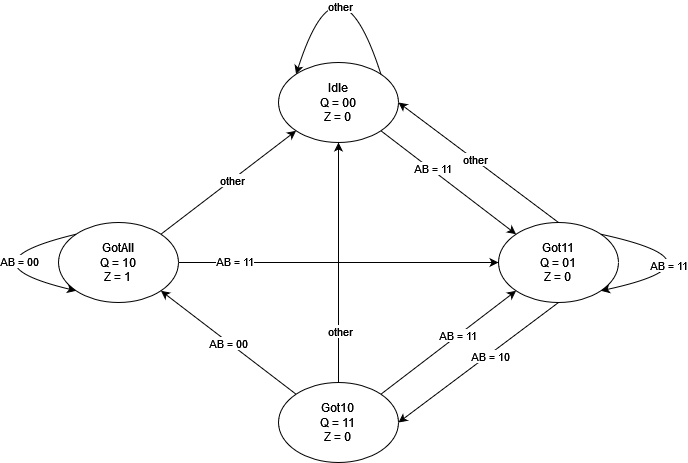
\includegraphics[scale=0.46]{statediagram.png}
\end{center}
\begin{center}
  Figure 1: \textit{State Diagram for the Sequence Detector}
\end{center}

Figure 1 shows how each state leads to the next and under what conditions. This helped to solidify
the exact behavior of the state machine.
In order to turn this concept into a circuit, a state table was created based upon the state diagram, shown in Table 1.

\begin{center}
  Table 1: \textit{State Table for the Sequence Detector}
\end{center}
\begin{center}
  \begin{NiceTabular}{|c||c|c||c|c||c|c||c|}
    \hline
    $RST$ & $Q_1$ & $Q_0$ & $A$ & $B$ & $Q_1^*$ & $Q_0^*$ & Z \\
    \hline
    \hline
    1 & * & * & * & * & 0 & 0 & 0 \\
    \hline
    0 & * & * & 1 & 1 & 0 & 1 & * \\
    \hline
    0 & 0 & 0 & * & * & * & * & 0 \\
    \hline
    0 & 0 & 1 & 1 & 0 & 1 & 1 & 0 \\
    \hline
    0 & 1 & 1 & 0 & 0 & 1 & 0 & 0 \\
    \hline
    0 & 1 & 0 & 0 & 0 & 1 & 0 & 1 \\
    \hline
    0 & * & * & * & * & 0 & 0 & * \\
    \hline
  \end{NiceTabular}
\end{center}

Table 1 shows the intended state changes that should occur within the state machine
when designed, and the last row represents that any conditions that were not previously
defined in other rows will always lead to the next state being Idle. In order to make the 
circuit design process simpler, this state table
was used to design boolean expressions that describe the state machine. Equations 1-3 describe
the state transitions and how the output $Z$ is defined.

\begin{align}
  Q_1^* = \overline{Q_1}Q_0A\overline{B} + Q_1\overline{A}\ \overline{B} \\
  Q_0^* = \overline{Q_1}Q_0A + AB \\
  Z = Q_1\overline{Q_0}
\end{align}

These equations define the next state of the state machine as a SOP expression of
the current state and the current inputs, allowing the entire state machine to be designed
around a SOP circuit using minterms. In Figure 2, a circuit designed around these equations is shown.

\begin{center}
  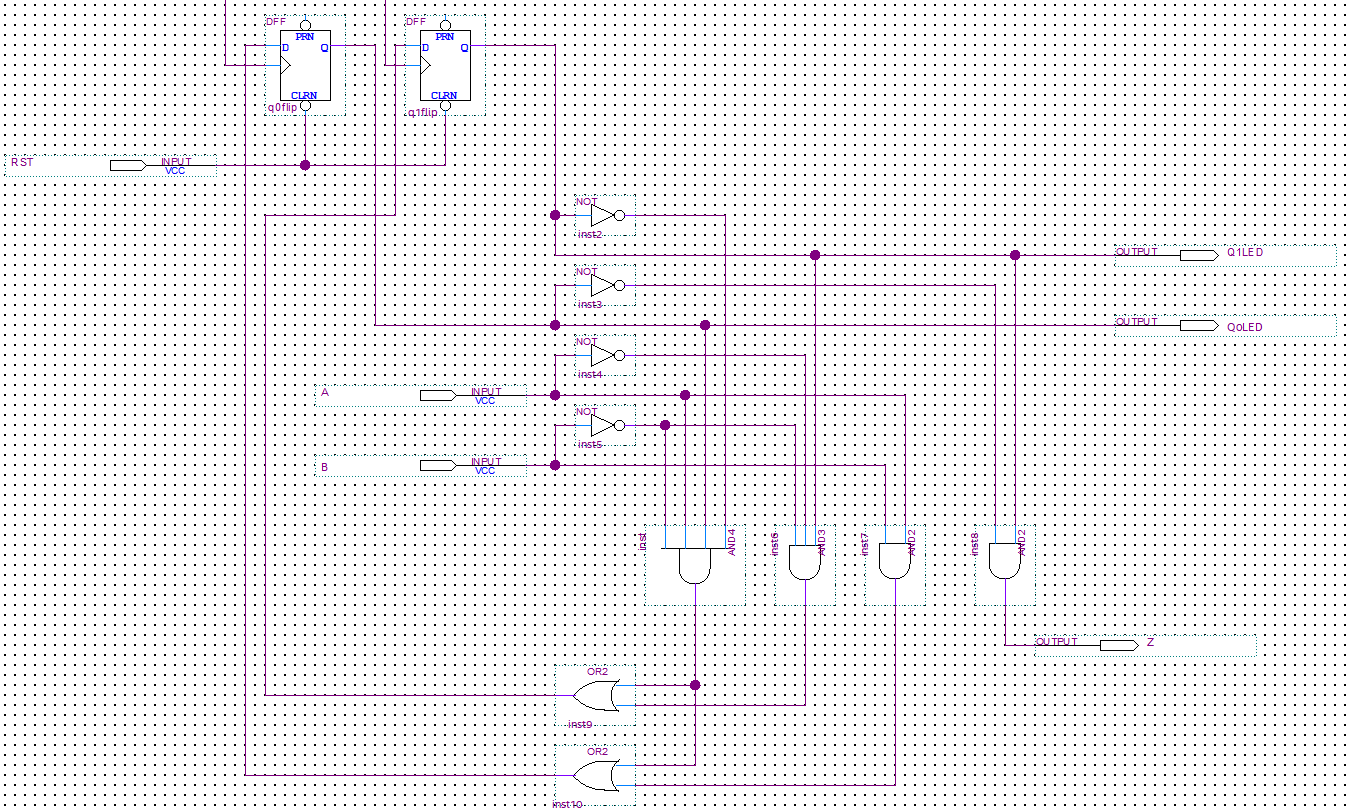
\includegraphics[scale=0.46]{circuit.png}
\end{center}
\begin{center}
  Figure 2: \textit{Implementation of a Sequence Detector in Quartus Prime}
\end{center}

Figure 2 displays the sequence detector as a circuit. It uses three minterms to define
the next state of the circuit and one to produce the output of the design. The minterm
for $\overline{Q_1}Q_0A$ in Equation 2 could be substituted with the existing minterm for 
$\overline{Q_1}Q_0A\overline{B}$, as the outputs are equivalent due to the other minterm in
Equation 2, $AB$.

The sequence detector
was implemented into the MAX10 FPGA by connecting 
the signals to the pins shown in Table 2. Two PLLs were
also used alongside a 50MHz clock signal to create a 2Hz clock for the clock inputs
on the D-flip-flops.

\begin{center}
  Table 2: \textit{Sequence Detector Pin to Signal Connections}
\end{center}
\begin{center}
  \begin{NiceTabular}{|c|c|}
    \hline
    Signal & MAX10 FPGA Pin \\
    \hline
    \hline
    $A$ & SW1 \\
    \hline
    $B$ & SW0 \\
    \hline
    $Q1LED$ & LEDR9 \\
    \hline
    $Q0LED$ & LEDR8 \\
    \hline
    $Z$ & LEDR0 \\
    \hline
    $clk\_50MHz$ & MAX10\_CLK1\_50 \\
    \hline
    $RST$ & KEY0 \\
    \hline
  \end{NiceTabular}
\end{center}

Table 2 shows the connections to the FPGA for the sequence detector. A hardware test verified that
the design operated correctly on the FPGA.
  
% \section*{Procedure}
% [\textit{Verify in the ``Lab Report'' section of the lab assignment
%   whether this section is required for this exercise.}]
% \par The procedure tells what was done and how it was done in a
%   chronological, narrative style--in contrast to a lab assignment’s
%   procedure section, which is typically written in imperative style,
%   (i.e., list of instructions).  The report’s procedure should tell in
%   the writer’s own words what was actually done in lab.  From reading
%   the procedure, the reader should be able to perform the exercise to
%   get the same results as the writer presents.

\break

\section*{Results and Analysis}
\par To verify the circuit built in Figure 2, the sequence detector circuit was simulated using ModelSim,
using two different sequences. The first of the input sequences produced the waveform shown in Figure 3.

\begin{center}
  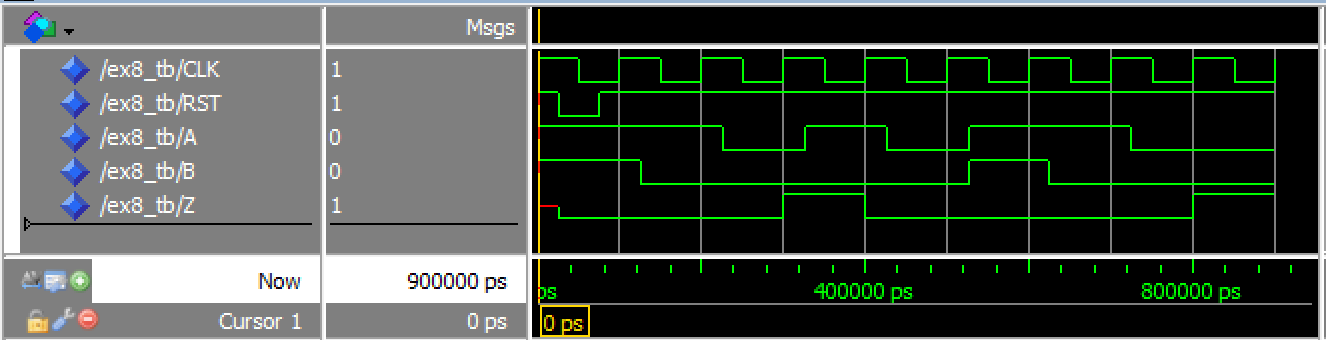
\includegraphics[scale=0.86]{theirwaves.png}
\end{center}
\begin{center}
  Figure 3: \textit{Waveforms Produced by the Sequence Detector in ModelSim for Sequence 1}
\end{center}


Figure 3 shows the waveform output of the sequence detector when the input sequence is 
(A,B) = (1,1), (1,0), (0,0), (1,0), (0,0), (1,1), (1,0), (0,0), (0,0). It demonstrates the
full sequence being detected for one clock cycle, and a partial sequence being detected later.
In order to test another feature of the detector, a second sequence was tested. The waveforms
produced when testing this second sequence are shown in Figure 4.

\begin{center}
  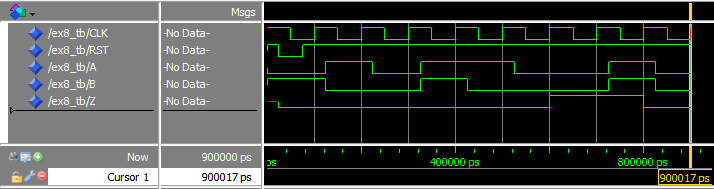
\includegraphics[scale=0.8]{ownwaves.png}
\end{center}
\begin{center}
  Figure 4: \textit{Waveforms Produced by the Sequence Detector in ModelSim for Sequence 2}
\end{center}

Figure 4 shows the waveform output of the sequence detector when the input sequence is
(A,B) = (0,1), (1,0), (0,0), (1,1), (1,0), (0,0), (0,0), (1,1), (0,0). This sequence
demonstrates how the detector's output continues to be high as long as the input continues
to be (A,B) = (0,0). The waveforms in Figures 3 and 4 demonstrate expected behavior and therefore
the exercise was successful.

\section*{Conclusion}

\par Sequence detectors are a very common part of modern electronics, although may sometimes be defined
in software rather than hardware. For example, the handshakes that happen at the beginning of many IO interactions,
like when a USB device is plugged in, use sequence detection in order to fully define what is happening and to set
a starting point for communications. This exercise was successful, as the sequence detector successfully performed
the operations expected and reacted to inputs as expected.

\break

\section*{Questions}
\par 1. Repeat the synthesis process of your state machine where Idle = 00, Got11 = 01, Got10 = 10, and GotAll = 11

The state diagram is almost the exact same, with the only change being that GotAll and Got10 have switched Q values.
Table 3 shows the new state table with the new encoding.

\begin{center}
  Table 3: \textit{State Table for the Sequence Detector with new encoding}
\end{center}
\begin{center}
  \begin{NiceTabular}{|c||c|c||c|c||c|c||c|}
    \hline
    $RST$ & $Q_1$ & $Q_0$ & $A$ & $B$ & $Q_1^*$ & $Q_0^*$ & Z \\
    \hline
    \hline
    1 & * & * & * & * & 0 & 0 & 0 \\
    \hline
    0 & * & * & 1 & 1 & 0 & 1 & * \\
    \hline
    0 & 0 & 0 & * & * & * & * & 0 \\
    \hline
    0 & 0 & 1 & 1 & 0 & 1 & 0 & 0 \\
    \hline
    0 & 1 & 0 & 0 & 0 & 1 & 1 & 0 \\
    \hline
    0 & 1 & 1 & 0 & 0 & 1 & 1 & 1 \\
    \hline
    0 & * & * & * & * & 0 & 0 & * \\
    \hline
  \end{NiceTabular}
\end{center}

Table 3 shows the new state table. Using this new state table, new equations can be made. Equations 4-6
show these new equations.

\begin{align}
  Q_1^* = \overline{Q_1}Q_0A\overline{B} + Q_1\overline{A}\ \overline{B} \\
  Q_0^* = Q_1\overline{A}\ \overline{B} + AB \\
  Z = Q_1Q_0
\end{align}

Equations 4-6 show that $Q_1^*$ is unchanged, and $Z$ and $Q_1^*$ are slightly modified to fit the new table.

\vspace{15pt}

\par 2. How many different ways are there to encode a state machine with four states that is implemented using
two D-flip flops? Note that the answer should be a number, not "one-hot" or "gray".

A state machine with four states and two D-flip flops could be encoded $4 * 3 * 2 * 1 = 24$ different ways.

\vspace{15pt}

\par 3. What is "one-hot" encoding style?

"One-hot" encoding is when a single bit is high for each individual state, and thus requires the same number
of bits as states.

\vspace{15pt}

\label{LastPage}
\end{document}